% Options for packages loaded elsewhere
\PassOptionsToPackage{unicode}{hyperref}
\PassOptionsToPackage{hyphens}{url}
%
\documentclass[
]{article}
\title{W241 Final Project: Assessing Gender Bias in Educational Videos}
\author{Elizabeth Khan, Estrella Ndrianasy, Chandni Shah, Michelle Shen,
Catherine Tsai}
\date{}

\usepackage{amsmath,amssymb}
\usepackage{lmodern}
\usepackage{iftex}
\ifPDFTeX
  \usepackage[T1]{fontenc}
  \usepackage[utf8]{inputenc}
  \usepackage{textcomp} % provide euro and other symbols
\else % if luatex or xetex
  \usepackage{unicode-math}
  \defaultfontfeatures{Scale=MatchLowercase}
  \defaultfontfeatures[\rmfamily]{Ligatures=TeX,Scale=1}
\fi
% Use upquote if available, for straight quotes in verbatim environments
\IfFileExists{upquote.sty}{\usepackage{upquote}}{}
\IfFileExists{microtype.sty}{% use microtype if available
  \usepackage[]{microtype}
  \UseMicrotypeSet[protrusion]{basicmath} % disable protrusion for tt fonts
}{}
\makeatletter
\@ifundefined{KOMAClassName}{% if non-KOMA class
  \IfFileExists{parskip.sty}{%
    \usepackage{parskip}
  }{% else
    \setlength{\parindent}{0pt}
    \setlength{\parskip}{6pt plus 2pt minus 1pt}}
}{% if KOMA class
  \KOMAoptions{parskip=half}}
\makeatother
\usepackage{xcolor}
\IfFileExists{xurl.sty}{\usepackage{xurl}}{} % add URL line breaks if available
\IfFileExists{bookmark.sty}{\usepackage{bookmark}}{\usepackage{hyperref}}
\hypersetup{
  pdftitle={W241 Final Project: Assessing Gender Bias in Educational Videos},
  pdfauthor={Elizabeth Khan, Estrella Ndrianasy, Chandni Shah, Michelle Shen, Catherine Tsai},
  hidelinks,
  pdfcreator={LaTeX via pandoc}}
\urlstyle{same} % disable monospaced font for URLs
\usepackage[margin=1in]{geometry}
\usepackage{longtable,booktabs,array}
\usepackage{calc} % for calculating minipage widths
% Correct order of tables after \paragraph or \subparagraph
\usepackage{etoolbox}
\makeatletter
\patchcmd\longtable{\par}{\if@noskipsec\mbox{}\fi\par}{}{}
\makeatother
% Allow footnotes in longtable head/foot
\IfFileExists{footnotehyper.sty}{\usepackage{footnotehyper}}{\usepackage{footnote}}
\makesavenoteenv{longtable}
\usepackage{graphicx}
\makeatletter
\def\maxwidth{\ifdim\Gin@nat@width>\linewidth\linewidth\else\Gin@nat@width\fi}
\def\maxheight{\ifdim\Gin@nat@height>\textheight\textheight\else\Gin@nat@height\fi}
\makeatother
% Scale images if necessary, so that they will not overflow the page
% margins by default, and it is still possible to overwrite the defaults
% using explicit options in \includegraphics[width, height, ...]{}
\setkeys{Gin}{width=\maxwidth,height=\maxheight,keepaspectratio}
% Set default figure placement to htbp
\makeatletter
\def\fps@figure{htbp}
\makeatother
\setlength{\emergencystretch}{3em} % prevent overfull lines
\providecommand{\tightlist}{%
  \setlength{\itemsep}{0pt}\setlength{\parskip}{0pt}}
\setcounter{secnumdepth}{-\maxdimen} % remove section numbering
\usepackage{float}
\usepackage{booktabs}
\usepackage{longtable}
\usepackage{array}
\usepackage{multirow}
\usepackage{wrapfig}
\usepackage{float}
\usepackage{colortbl}
\usepackage{pdflscape}
\usepackage{tabu}
\usepackage{threeparttable}
\usepackage{threeparttablex}
\usepackage[normalem]{ulem}
\usepackage{makecell}
\usepackage{xcolor}
\ifLuaTeX
  \usepackage{selnolig}  % disable illegal ligatures
\fi

\begin{document}
\maketitle

{
\setcounter{tocdepth}{2}
\tableofcontents
}
\clearpage

\hypertarget{background}{%
\subsection{Background}\label{background}}

Female instructors face challenges with gender stereotypes that can
impact their future earning potentials and career growth. Specifically
for women in academia, numerous studies have demonstrated that students
treat and evaluate female professors differently than male professors.
Female professors are also often held to higher standards and subjected
to a greater number of demands and requests from their students.{[}2{]}
In this experiment, we seek to understand if gender bias alters
students' perception of an instructor's quality of programming and
technical instruction.

\hypertarget{research-questions}{%
\subsection{Research Questions}\label{research-questions}}

Primary Research Question: \emph{Does an instructor's perceived gender
influence the perceived quality of instruction?}

Secondary Research Question: \emph{Does an instructor's perceived gender
influence retention of content?}

\hypertarget{hypothesis}{%
\subsection{Hypothesis}\label{hypothesis}}

We hypothesize that the treatment of changing perceived gender of the
instructor will impact the measured instructor ratings from students due
to historical evidence of gender bias in academia favoring men's
performance, grant and award-winning potential, resource allocation, and
tenure that continues to reinforce gender wage gaps and lead to better
career outcomes for men. Specifically, in an academic learning setting,
we suspect that implicit gender biases against women can be observed
when evaluating instructor performance by exposing the treatment group
to instructors they perceive as female.

\hypertarget{data}{%
\subsection{Data}\label{data}}

To conduct the experiment, we explored subject recruiting companies in
order to obtain a more generalizable pool of survey participants. The
requirements outlined for recruiting companies included the ability to:

\begin{itemize}
\tightlist
\item
  Administer Qualtrics survey to subjects
\item
  Record subject responses
\item
  Ensure sufficient sample size according to our power analysis (see
  Statistical Analysis Approach)
\item
  Enable blocked design
\item
  Include inclusion and exclusion criteria
\item
  Disqualify those who failed the attention check
\item
  Deliver responses to us in a timely manner
\end{itemize}

The social science recruitment company we chose to work with,
SurveySwap, was the best fit based on the criteria above. SurveySwap was
used to identify subjects, deliver control and treatment surveys, and
deliver subject responses.

\hypertarget{experiment-design}{%
\subsection{Experiment Design}\label{experiment-design}}

Our experiment featured a randomized, between-subjects design with a 2x4
blocked design on the gender and age groups of participants so as to
ensure equal treatment distribution among each of the blocked
populations. The sample design consisted of 112 participants equally
split between self-identified males (n = 56) and females (n = 56) survey
participants.

The control group consisted of subjects who visualized a Python
instructional video voiced using a male voiceover. The treatment group
were subjects who watched the exact same video voiced using a female
instead of a male voiceover. To further mitigate potential
instructor-level attributes that may influence instructor evaluations,
subjects in the treatment and control groups were randomly assigned to
one of three possible instructors. Specifically, there were six
different recordings of the same video with the same script in the
experiment: three different male recordings within the control group,
and three different female ones in the treatment group.

Subjects were sorted into blocks (Table 1) and then randomized into
surveys utilizing Qualtrics's survey logic functions. The
\textbf{\emph{primary outcome}} variables were:

\begin{itemize}
\tightlist
\item
  \textbf{Enthusiasm}: rating of the instructor's enthusiasm
\item
  \textbf{Knowledge}: rating of the instructor's knowledge
\item
  \textbf{Clarity}: rating on how clearly respondents felt the
  instructor explained the material
\item
  \textbf{Professionalism}: evaluating the instructor's professionalism
\item
  \textbf{Overall Effectiveness}: rating of the overall effectiveness of
  the instructor's teaching
\end{itemize}

Primary outcome variable questions were administered as questions using
a 5-point Likert scale. A secondary outcome variable was \textbf{quiz
score} measured on the correctness of answers to several content
retention questions. The inclusion and exclusion criteria requirements
detailed below were stipulated to allow researchers to capture treatment
effects for adults in the United States.

\textbf{Inclusion criteria:} To qualify for the survey, subjects must be
located in the United States and identify as a native English speaker.

\textbf{Exclusion criteria:} Subjects less than 20 years of age were
excluded from the study.

\begin{center}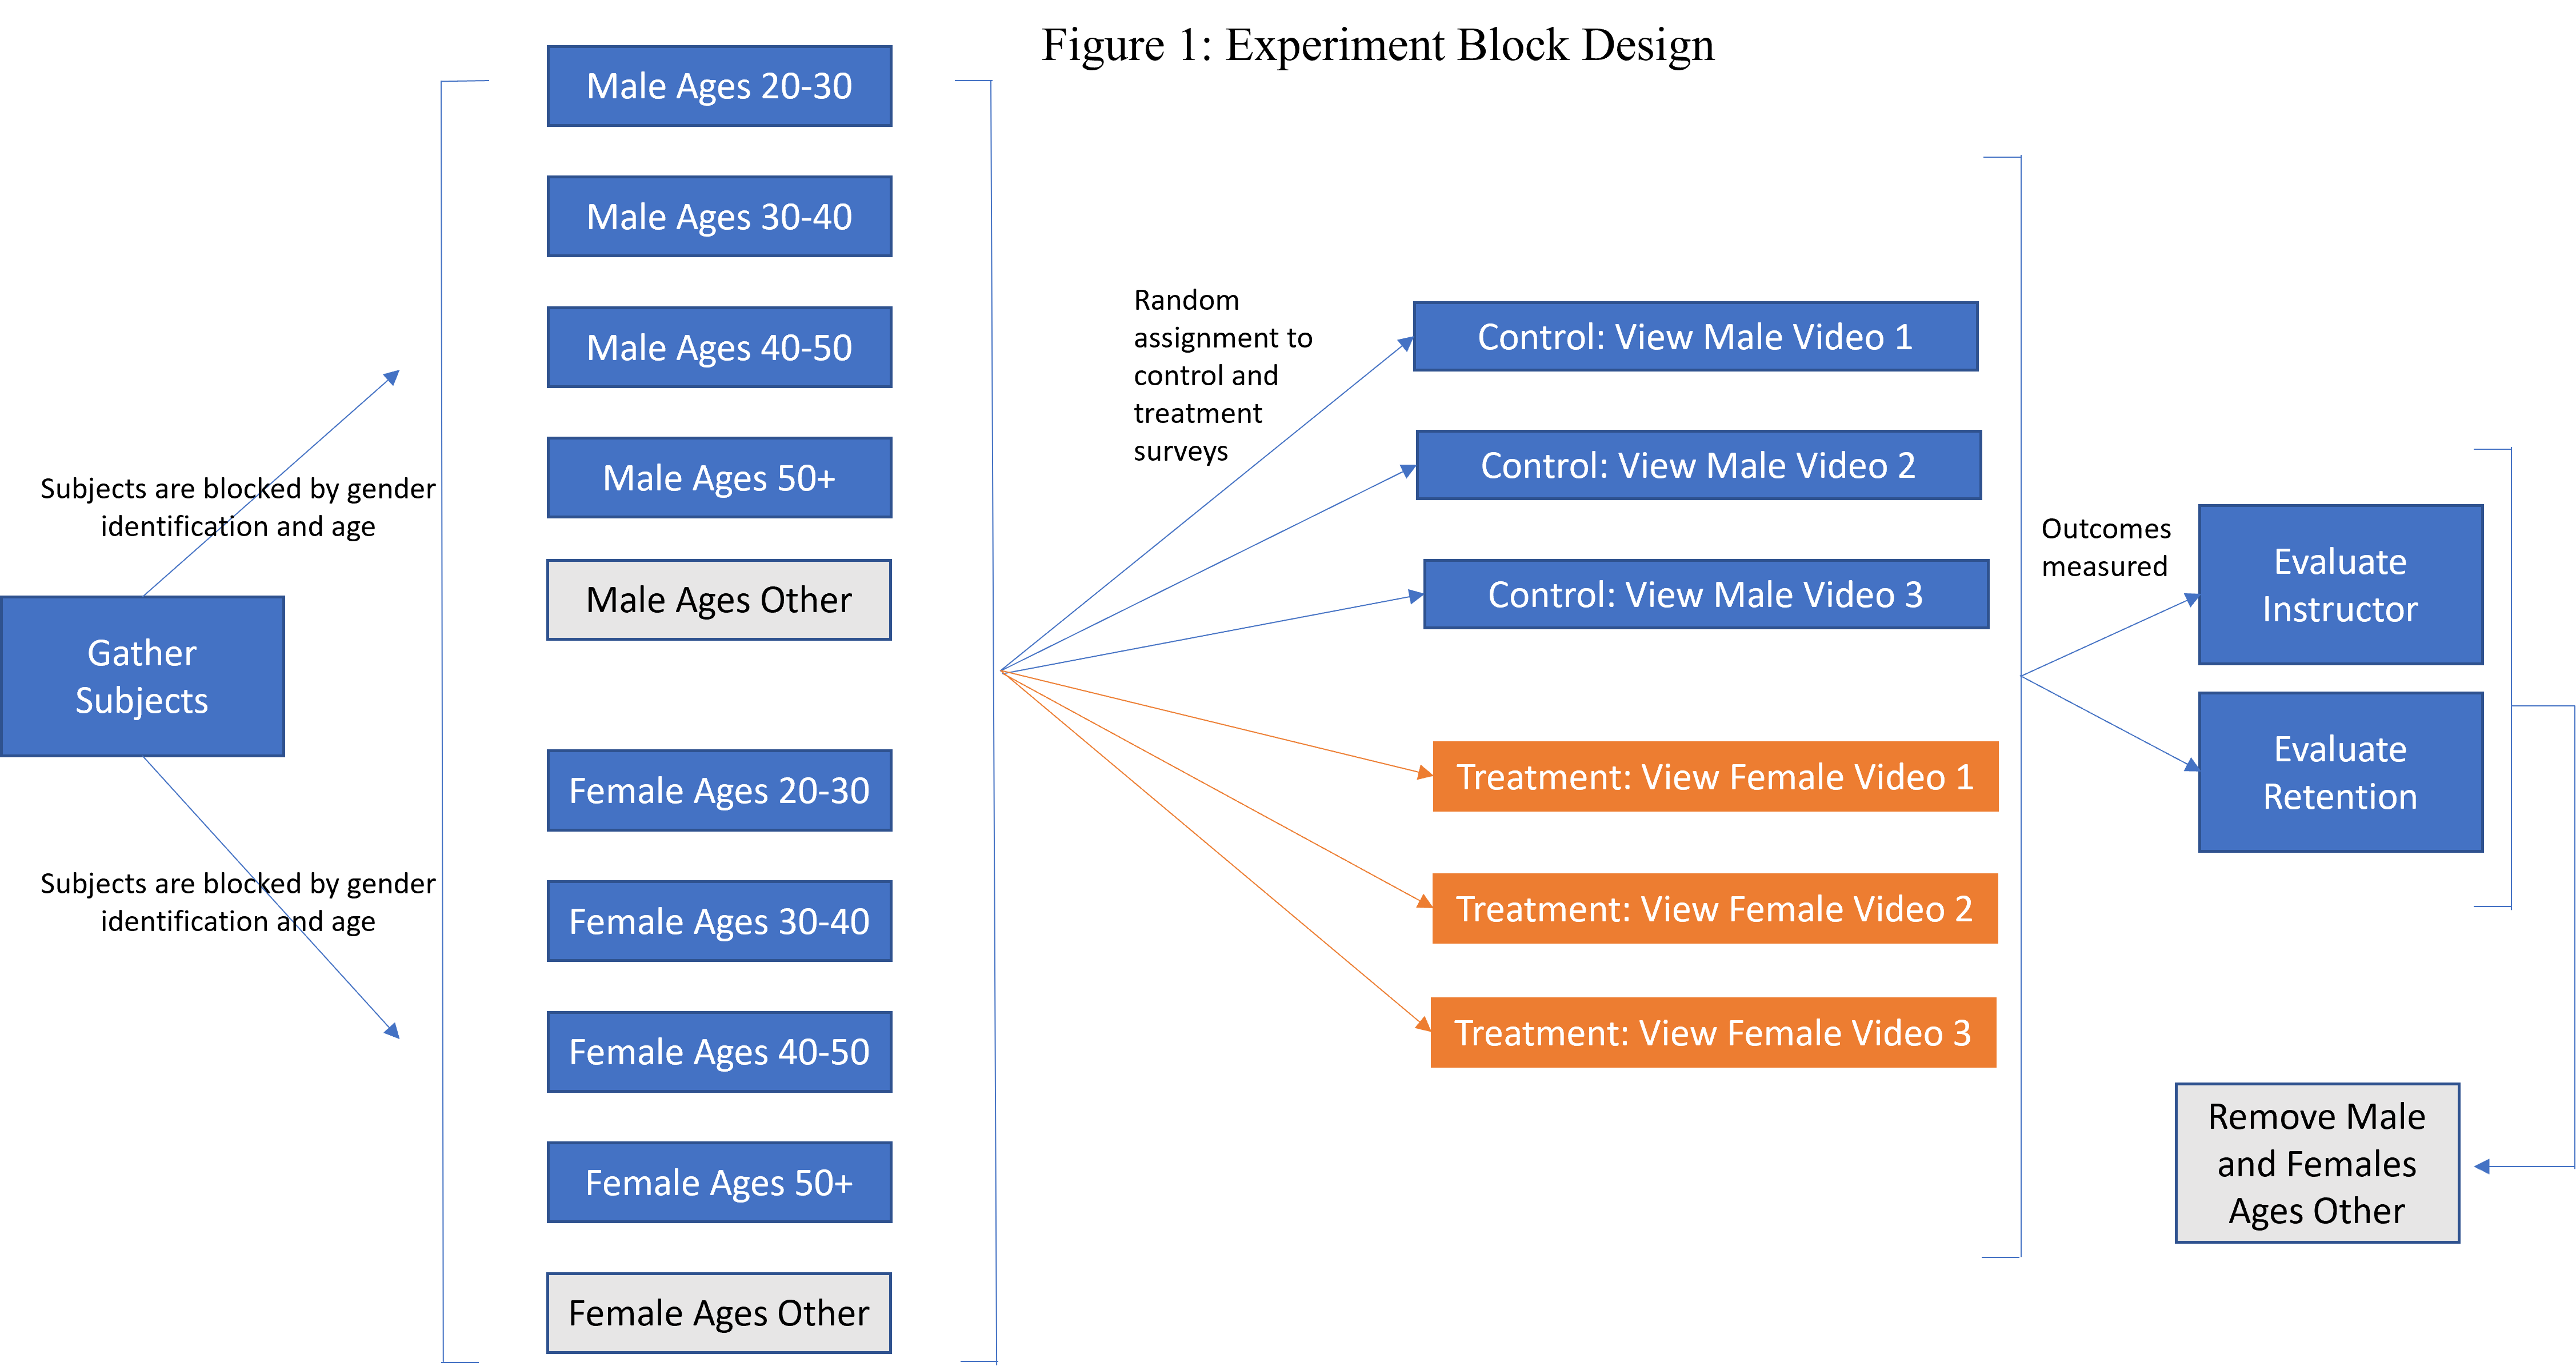
\includegraphics[width=0.9\linewidth,height=0.9\textheight]{images/ExperimentalDesign} \end{center}

\hypertarget{statistical-power}{%
\subsection{Statistical Power}\label{statistical-power}}

Prior to conducting the experiment, a statistical power test was
completed to evaluate whether a sample size of at least 112
participants, evenly split between treatment and control, would be
sufficient to observe the treatment effect. It was estimated from the
average outcome from the Gender Bias in Student Evaluations Study by
Kristina Mitchell and Johnathan Martin {[}3{]}. The test showed 95\% of
all potential random assignments would effectively reject the null
hypothesis in the presence of a treatment effect. Therefore, a sample
size of at least 112 is presumed sufficient.

\hypertarget{potential-outcomes-and-reasoning-about-mechanisms}{%
\subsection{Potential Outcomes and Reasoning About
Mechanisms}\label{potential-outcomes-and-reasoning-about-mechanisms}}

To understand the causal effect of the treatment we used the Potential
Outcomes framework in order to estimate the Average Treatment Effect
(ATE). For the purposes of this study we compared two potential outcomes
1) \(Y_i(1)\) which is the observed outcome (instructor rating) when the
subject watches the video with a female instructor and 2) \(Y_i(0)\) the
observed outcome (instructor rating) when the subject watches the video
with a male instructor.

The delivered treatment (\(d_i=1\)) of changing instructor gender to
female is used as a means to quantify the differences in perception
between male and female instructors. The videos would allow the students
to infer the perceived genders of the instructors along with the style
and assumed content mastery. Because male instructed videos will be used
as a control, it can be used to establish a baseline of instructor
perception. The perception by the treatment group watching videos led by
a female instructor might deviate from that baseline. If there are
significant differences between the control and treatment group, holding
the content of the material and everything else except gender constant,
then we can attribute that the gender of the instructor leads to
differences between the control and treatment outcomes .

\hypertarget{statistical-analysis-approach}{%
\subsection{Statistical Analysis
Approach}\label{statistical-analysis-approach}}

The Average Treatment Effect (ATE) of receiving the Male Instructor
Video on the outcome will be estimated using Linear Regression models.
Specifically, the experiment analyzed five (5) primary outcomes and one
secondary outcome.

\textbf{Model 1}: The simple model estimates the ATE of the receiving
the treatment (Female Instructor Video) as compared to the control group
(Male Instructor Video).

\(Outcome=\beta_0+\beta_1 Female Instructor Video\)

\textbf{Model 2}: The second model includes blocks for subject Age and
Gender. We theorized the potential outcomes would be similar for the
Gender and Age group. Additionally, this model enables the comparison of
the ATE among the male group, the ATE among the female group, and the
ATE for various Age Groups of respondents.

\(Outcome=\beta_0+\beta_1 Female Instructor Video \ +\beta_2Age:30-40\ +\beta_3Age:40-50\ +\beta_4Age:50+\beta_5Male\)

\textbf{Model 3}: The third model includes interaction terms for Gender
and Treatment (Female Instructor Video) in addition to the block
covariates because there is reason to suspect that Gender may have an
additional effect on the receiving the treatment. Specifically, males
may evaluate female instructors lower than male instructors because of
gender bias.

\(Outcome=\beta_0+\beta_1 Female Instructor Video \ +\beta_2Age:30-40\ +\beta_3Age:40-50\ +\beta_4Age:50+\beta_5Male +\beta_6(Male*FemaleInstructorVideo)\)

\hypertarget{methodology}{%
\subsection{Methodology}\label{methodology}}

\hypertarget{survey-development}{%
\subsubsection{Survey Development}\label{survey-development}}

A video featuring a Python programming informational slideshow was
created. To control for cadence, pitch, tone, and other characteristics
that vary among both men's and women's voices, a total of six voiceovers
from three (3) male and three female (3) volunteers were recorded to
narrate the same video. Volunteers used the same script and were given
timestamps to standardize the pacing of the six (6) resulting videos.
Neither videos nor images of volunteers were incorporated into the final
videos. Namely, no identifiable information on the volunteers was made
available to the survey participants.

A questionnaire containing thirteen (13) survey questions (see Appendix
A) was generated to collect information on two main outcomes. First, the
subject was asked three (3) demographics questions about the subject's
gender, age group, and highest level of education. Next, five (5)
primary outcome questions to collect information on instructor
perception from the video. Primary outcome questions use a 5-point
Likert Scale for subjects to rate the quality of the instructor's
performance. One (1) attention check question was administered at this
time. Next, the subject is asked four (4) secondary objective outcome
questions to test video content retention among respondents. Questions
were presented in multiple-choice format with one correct response.

Six Qualtrics surveys were generated. Each Qualtrics survey contained
only one of the six videos with either a male or a female voiceover,
followed by the questionnaire. A 10 second timer was added to each page
of the survey.

\hypertarget{treatment-adminstration}{%
\subsubsection{Treatment Adminstration}\label{treatment-adminstration}}

SurveySwap recruited subjects based on established blocks for gender and
age group (Figure 1). After answering demographic questions, subjects
were randomized to one of the six surveys in accordance with blocking
per the experimental design. Within the survey, subjects were asked to
view a video and fill out survey questions. Only the survey responses
from subjects that correctly answered the attention check question were
recorded.

\hypertarget{survey-outcomes}{%
\subsection{Survey Outcomes}\label{survey-outcomes}}

\begin{center}\includegraphics[width=0.9\linewidth,height=0.9\textheight]{images/consort} \end{center}

\hypertarget{subject-demographics}{%
\subsection{Subject Demographics}\label{subject-demographics}}

SurveySwap provided data from 223 total subjects (see Table 1). Of those
subjects, 49\% were assigned to the control group and 51\% were assigned
to the treatment group. Our findings show that 63\% of respondents only
achieved a high school degree or some college (see Table 2). A majority
of respondents (64\%) were also self identified as female. This
education and gender imbalance was highlighted as survey results and
potential interpretation may be impacted (see Table 2). The following
tables show the full summary of subjects within each gender and age
block, along with educational attainment.

\begin{table}[H]

\caption{\label{tab:table1_2}Respondents by Age Group and Gender}
\centering
\begin{tabular}[t]{l|l|l|l}
\hline
Characteristic & Overall, N = 223 & Female, N = 143 & Male, N = 80\\
\hline
assignment &  &  & \\
\hline
\hspace{1em}Control & 109 (49\%) & 69 (48\%) & 40 (50\%)\\
\hline
\hspace{1em}Treatment & 114 (51\%) & 74 (52\%) & 40 (50\%)\\
\hline
Age &  &  & \\
\hline
\hspace{1em}20-30 & 44 (20\%) & 25 (17\%) & 19 (24\%)\\
\hline
\hspace{1em}30-40 & 82 (37\%) & 56 (39\%) & 26 (32\%)\\
\hline
\hspace{1em}40-50 & 48 (22\%) & 32 (22\%) & 16 (20\%)\\
\hline
\hspace{1em}50+ & 47 (21\%) & 29 (20\%) & 18 (22\%)\\
\hline
\hspace{1em}Other & 2 (0.9\%) & 1 (0.7\%) & 1 (1.2\%)\\
\hline
\multicolumn{4}{l}{\rule{0pt}{1em}\textsuperscript{1} n (\%)}\\
\multicolumn{4}{l}{\textsuperscript{a} Note: The two subjects with Age='Other' will be excluded because they meet}\\
\multicolumn{4}{l}{exclusion criteria}\\
\end{tabular}
\end{table}

\begin{table}[H]

\caption{\label{tab:table1_2}Respondents by Education and Treatment Assignment}
\centering
\begin{tabular}[t]{l|l|l|l}
\hline
Characteristic & Overall, N = 223 & Control, N = 109 & Treatment, N = 114\\
\hline
Gender &  &  & \\
\hline
\hspace{1em}Female & 143 (64\%) & 69 (63\%) & 74 (65\%)\\
\hline
\hspace{1em}Male & 80 (36\%) & 40 (37\%) & 40 (35\%)\\
\hline
Education &  &  & \\
\hline
\hspace{1em}Associates degree & 27 (12\%) & 16 (15\%) & 11 (9.6\%)\\
\hline
\hspace{1em}Bachelors degree & 43 (19\%) & 21 (19\%) & 22 (19\%)\\
\hline
\hspace{1em}High school diploma & 67 (30\%) & 34 (31\%) & 33 (29\%)\\
\hline
\hspace{1em}Less than High school & 7 (3.1\%) & 1 (0.9\%) & 6 (5.3\%)\\
\hline
\hspace{1em}Masters degree & 12 (5.4\%) & 5 (4.6\%) & 7 (6.1\%)\\
\hline
\hspace{1em}Some College No degree & 67 (30\%) & 32 (29\%) & 35 (31\%)\\
\hline
\multicolumn{4}{l}{\rule{0pt}{1em}\textsuperscript{1} n (\%)}\\
\multicolumn{4}{l}{\textsuperscript{a} Note: The two subjects with Age='Other' will be excluded because they meet exclusion}\\
\multicolumn{4}{l}{criteria}\\
\end{tabular}
\end{table}

\hypertarget{confirmation-of-randomization-and-covariate-balancing}{%
\subsection{Confirmation of Randomization and Covariate
Balancing}\label{confirmation-of-randomization-and-covariate-balancing}}

An F-test was conducted in R to evaluate whether the subjects were
randomly assigned to the control and treatment group based on age and
gender blocks. We fail to reject the null hypothesis with a
non-statistically significant p-value of 0.795. Moreover, the F-test
results indicate there is no evidence supporting the addition of block
covariates would increase the accuracy of predicting treatment exposure,
and that the blocks were successfully randomized.

\hypertarget{pre-treatment-covariates}{%
\subsubsection{Pre-Treatment
Covariates}\label{pre-treatment-covariates}}

We hypothesized gender, age, and level of education of subjects may
influence the outcomes measured. A separate covariate balance check was
conducted to evaluate the differences in means between the treatment and
control groups for the pretreatment characteristics. We subsequently
found no imbalance between pre-treatment covariates, as none of the
p-values were statistically significant.

\begin{longtable}[]{@{}
  >{\raggedright\arraybackslash}p{(\columnwidth - 10\tabcolsep) * \real{0.29}}
  >{\raggedright\arraybackslash}p{(\columnwidth - 10\tabcolsep) * \real{0.15}}
  >{\raggedright\arraybackslash}p{(\columnwidth - 10\tabcolsep) * \real{0.16}}
  >{\raggedright\arraybackslash}p{(\columnwidth - 10\tabcolsep) * \real{0.12}}
  >{\raggedright\arraybackslash}p{(\columnwidth - 10\tabcolsep) * \real{0.14}}
  >{\raggedright\arraybackslash}p{(\columnwidth - 10\tabcolsep) * \real{0.14}}@{}}
\caption{Covariate Balance Test}\tabularnewline
\toprule
\begin{minipage}[b]{\linewidth}\raggedright
\end{minipage} & \begin{minipage}[b]{\linewidth}\raggedright
Control (N = 108)
\end{minipage} & \begin{minipage}[b]{\linewidth}\raggedright
Treatment (N = 113)
\end{minipage} & \begin{minipage}[b]{\linewidth}\raggedright
Mean - Control
\end{minipage} & \begin{minipage}[b]{\linewidth}\raggedright
Mean - Treatment
\end{minipage} & \begin{minipage}[b]{\linewidth}\raggedright
t-test (p-value)
\end{minipage} \\
\midrule
\endfirsthead
\toprule
\begin{minipage}[b]{\linewidth}\raggedright
\end{minipage} & \begin{minipage}[b]{\linewidth}\raggedright
Control (N = 108)
\end{minipage} & \begin{minipage}[b]{\linewidth}\raggedright
Treatment (N = 113)
\end{minipage} & \begin{minipage}[b]{\linewidth}\raggedright
Mean - Control
\end{minipage} & \begin{minipage}[b]{\linewidth}\raggedright
Mean - Treatment
\end{minipage} & \begin{minipage}[b]{\linewidth}\raggedright
t-test (p-value)
\end{minipage} \\
\midrule
\endhead
\textbf{Gender} & ~~ & ~~ & ~~ & ~~ & ~~ \\
~~ Male & 40 (37.04\%) & 39 (34.51\%) & 0.37 & 0.35 & 0.697 \\
~~ Female & 68 (62.96\%) & 74 (65.49\%) & 0.63 & 0.65 & 0.697 \\
\textbf{Age} & ~~ & ~~ & ~~ & ~~ & ~~ \\
~~ 20-30 & 23 (21.30\%) & 21 (18.58\%) & 0.21 & 0.19 & 0.616 \\
~~ 30-40 & 39 (36.11\%) & 43 (38.05\%) & 0.36 & 0.38 & 0.766 \\
~~ 40-50 & 26 (24.07\%) & 22 (19.47\%) & 0.24 & 0.19 & 0.41 \\
~~ 50+ & 20 (18.52\%) & 27 (23.89\%) & 0.19 & 0.24 & 0.33 \\
\textbf{Education} & ~~ & ~~ & ~~ & ~~ & ~~ \\
~~ Less than High school & 1 (0.93\%) & 6 (5.31\%) & 0.01 & 0.05 & NA \\
~~ High school diploma & 33 (30.56\%) & 33 (29.20\%) & 0.31 & 0.29 &
0.827 \\
~~ Some College No degree & 32 (29.63\%) & 35 (30.97\%) & 0.3 & 0.31 &
0.829 \\
~~ Associates degree & 16 (14.81\%) & 11 (9.73\%) & 0.15 & 0.1 &
0.253 \\
~~ Bachelors degree & 21 (19.44\%) & 22 (19.47\%) & 0.19 & 0.19 &
0.996 \\
~~ Masters degree & 5 (4.63\%) & 6 (5.31\%) & 0.05 & 0.05 & 0.817 \\
\bottomrule
\end{longtable}

\hypertarget{empirical-data}{%
\subsection{Empirical Data}\label{empirical-data}}

Our primary outcome analysis explores the distribution of Overall
Instructor Effectiveness ratings and each of the five instructor ratings
separately. The mean instructor overall rating is 3.5 for the treatment
group and 3.6 for the control. While the distribution of control and
treatment groups are slightly skewed to the left, we observe the
majority of subjects in the control group who viewed a male instructor
rated the overall instructor effectiveness 4 out of 5. On the other
hand, the majority of subjects in the treatment group who viewed a
female instructor rated the instructor 3 out of 5 (see Figure 3).

As shown in Figure 4, the average ratings for the treatment group and
control group are 3.14 vs.~2.78 (Enthusiasm), 3.82 vs.~3.78
(Professional), 3.93 vs.~3.86 (Knowledge), 3.81 vs.~3.63 (Clarity), and
3.5 vs.~3.6 (Overall Effectiveness) respectively. The standard error
bars (95\% CIs) largely overlap across the treatment and control groups
for all ratings except for Instructor Enthusiasm. This suggests that
there may be a meaningful difference between the treatment and control
group for Instructor Enthusiasm. We will determine if this difference is
statistically significant in our subsequent regression analysis.

\begin{center}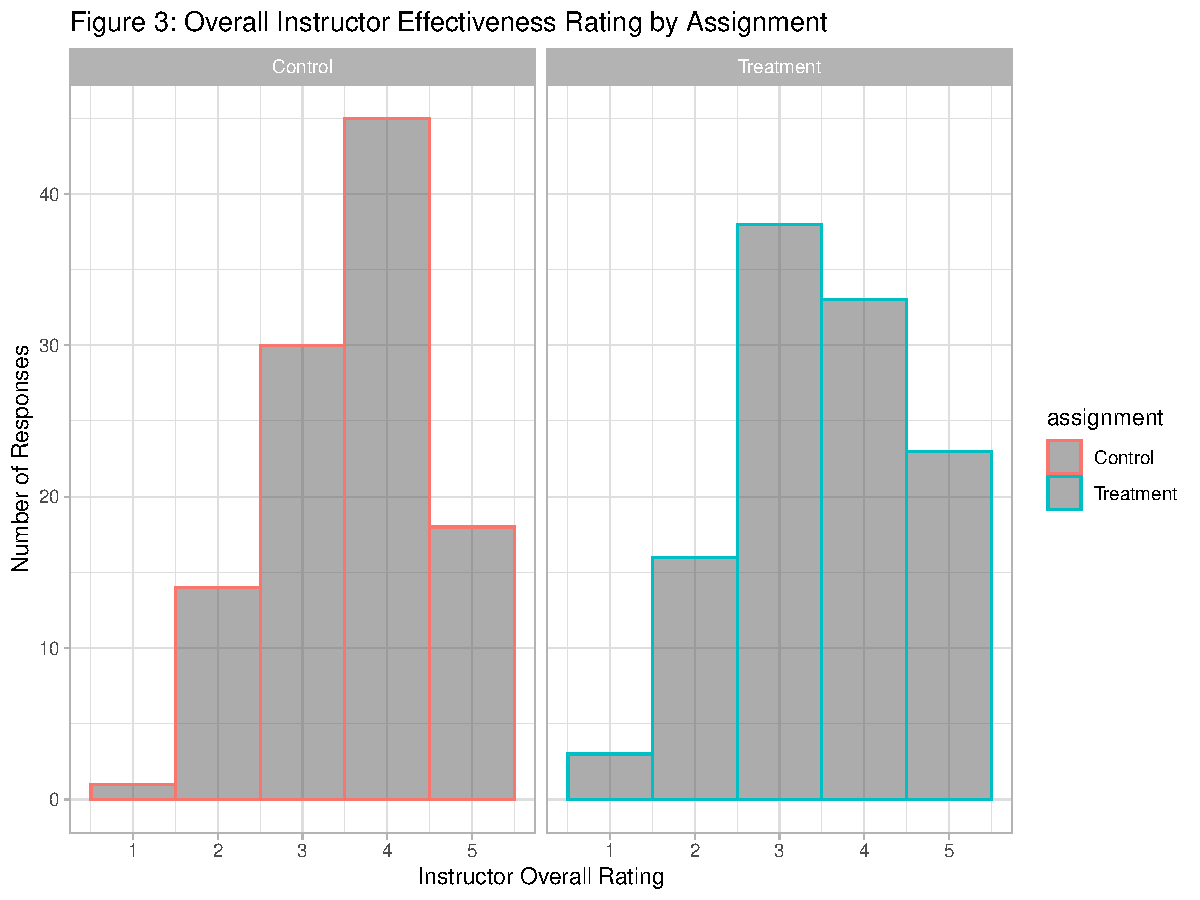
\includegraphics[width=0.8\linewidth]{final_project_markdown_files/figure-latex/unnamed-chunk-1-1} \end{center}

\begin{center}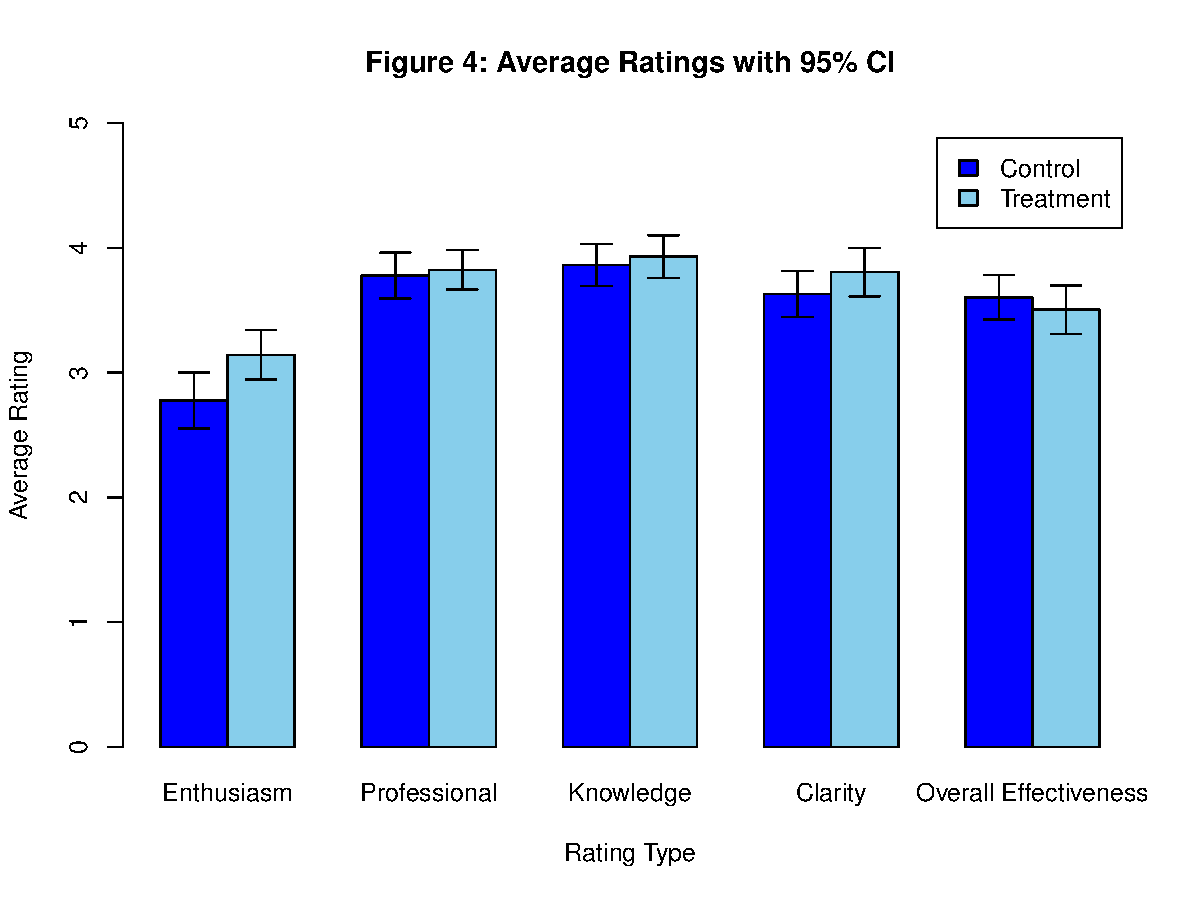
\includegraphics[width=0.8\linewidth]{final_project_markdown_files/figure-latex/unnamed-chunk-1-2} \end{center}

Our secondary outcome analysis explores content retention of subjects in
the control and treatment groups. The average quiz score for the
treatment group is 42.9\% and 44.9\% for the control. The overall quiz
scores are normally distributed around a score of 50\%, meaning the
majority of subjects answered 2 out of the 4 retention questions
correctly (see Figure 5 below).

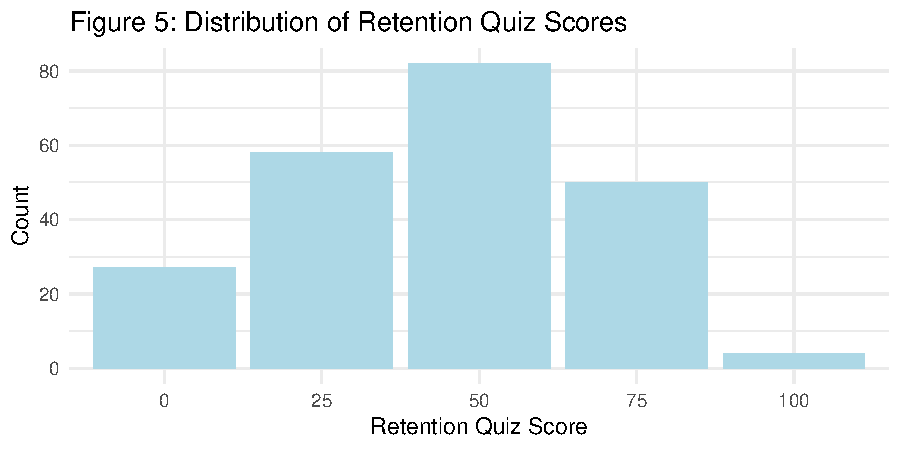
\includegraphics{final_project_markdown_files/figure-latex/unnamed-chunk-2-1.pdf}

\hypertarget{regressions}{%
\subsection{Regressions}\label{regressions}}

To measure the estimated treatment effect on our primary outcome
variables (Overall Instructor Effectiveness, Professionalism, Knowledge,
Material, Clarity, and Enthusiasm Rating) and our secondary outcome
variable (Quiz Score), we used three regression models (as described in
the Statistical Analysis Approach section). Additionally, we calculated
robust standard errors to estimate accurate errors without relying on
the assumption of homoskedastic errors.

\hypertarget{statistically-significant-results}{%
\subsubsection{Statistically Significant
Results}\label{statistically-significant-results}}

\textbf{Primary Outcome: Instructor Enthusiasm Rating}

Out of our five measured primary outcome variables and our single
measured secondary outcome variable, instructor enthusiasm was the only
variable with statistically significant results. Table 8 below shows the
results of the various regression models.

\textbf{Simple Model}

The Simple Model shows an ATE in Instructor Enthusiasm rating between
the treatment and control groups was 0.364, with a robust standard error
of 0.153 and a 95\% Confidence Interval of 0.0637 to 0.664. This
suggests that receiving the treatment of a female-perceived instructor
increases the instructor enthusiasm rating by 0.364 points. The Baseline
coefficient indicates that the control group who received a
male-perceived instructor had an average instructor enthusiasm rating of
2.78. We reject the null hypothesis that the treatment effect is equal
to zero as the Simple Model produces statistically significant results
(p-value = .018 \textless{} .05) for the ATE (Female Instructor beta
coefficient).

\textbf{Blocks Included Model}

The addition of the blocks for Age group and Gender minimally changes
the point estimate and precision for the Female Instructor Video
coefficient. Therefore, the treatment increases the instructor
enthusiasm rating by 0.369 points compared to the control group. In this
model, the baseline group includes only Female respondents between ages
20 to 30 that were in the control group. The intercept is the average
rating for the baseline group which is 2.68. The dummy variable block
for Age: 30-40 suggests a 0.043 points increase in rating as compared to
the 20-30 age group. The dummy variable block for Age: 40-50 suggests a
0.306 points decrease in the enthusiasm rating as compared to the 20-30
age group. The dummy variable block for Age: 50+ suggests a 0.114
decrease for the instructor enthusiasm rating compared to the 20-30 age
group. The dummy variable block for Gender (Male) suggests that
respondents who are males rate the instructor 0.479 points higher than
females. The treatment and Gender blocks produced statistically
significant results with a p-value of 0.0177 and 0.0003 respectively.
Therefore, we may reject the null hypothesis that the treatment effect
is equal to zero. Note: the Age group block coefficients are not
statistically significant.

\textbf{Gender Interaction Terms Model}

The last model introduces the interaction term which changes the point
estimate and changes the Female Instructor beta coefficient to 0.409
with a robust standard error of 0.193. This suggests that the treatment
increases the instructor enthusiasm rating by 0.409 points. The average
instructor enthusiasm rating for the baseline group is 2.67. The dummy
variable block for Age:30-40 suggests a 0.041 points increase compared
to the 20-30 age group. The Age: 40-50 dummy variable block suggests a
0.313 points decrease compared to the 20-30 age group. Lastly, the Age:
50+ suggests a 0.1147 points increase in the rating compared to the
20-30 age group. The dummy block variable for Gender(Male) suggests the
respondents who are males rate the professor 0.536 points higher than
females.The interaction term can be interpreted as the additional
increase in instructor rating that males subjects who receive the
treatment provide compared to female subjects, which is a 0.113 points
decrease in the instructor rating. As with the previous model, Age group
blocks and interaction terms are not statistically significant. The ATE
is statistically significant, therefore, we reject the null hypothesis
that the treatment effect on instructor enthusiasm of having a female
instructor is equal to zero.

\clearpage

\begin{table}[!htbp] \centering 
  \caption{Primary Outcome Instructor Enthusiasm Rating Models} 
  \label{} 
\small 
\begin{tabular}{@{\extracolsep{3pt}}lccc} 
\\[-1.8ex]\hline 
\hline \\[-1.8ex] 
 & \multicolumn{3}{c}{\textit{Dependent variable:}} \\ 
\cline{2-4} 
\\[-1.8ex] & \multicolumn{3}{c}{Enthusiasm Rating} \\ 
 & Simple & Blocks Included & Gender Interaction Terms \\ 
\\[-1.8ex] & (1) & (2) & (3)\\ 
\hline \\[-1.8ex] 
 Female Instructor Video & 0.364 & 0.369 & 0.409 \\ 
  & (0.153)$^{**}$ & (0.154)$^{**}$ & (0.193)$^{**}$ \\ 
  & p = 0.018 & p = 0.017 & p = 0.035 \\ 
  & & & \\ 
 Age: 30-40 &  & 0.043 & 0.041 \\ 
  &  & (0.218) & (0.219) \\ 
  &  & p = 0.846 & p = 0.853 \\ 
  & & & \\ 
 Age: 40-50 &  & $-$0.306 & $-$0.313 \\ 
  &  & (0.245) & (0.248) \\ 
  &  & p = 0.212 & p = 0.208 \\ 
  & & & \\ 
 Age: 50+ &  & $-$0.144 & $-$0.147 \\ 
  &  & (0.240) & (0.241) \\ 
  &  & p = 0.547 & p = 0.541 \\ 
  & & & \\ 
 Male &  & 0.479 & 0.536 \\ 
  &  & (0.157)$^{***}$ & (0.235)$^{**}$ \\ 
  &  & p = 0.003 & p = 0.023 \\ 
  & & & \\ 
 Male:Female Instructor Video &  &  & $-$0.113 \\ 
  &  &  & (0.319) \\ 
  &  &  & p = 0.723 \\ 
  & & & \\ 
 Baseline & 2.780 & 2.680 & 2.670 \\ 
  & (0.115)$^{***}$ & (0.205)$^{***}$ & (0.212)$^{***}$ \\ 
  & p = 0.000 & p = 0.000 & p = 0.000 \\ 
  & & & \\ 
\hline \\[-1.8ex] 
Observations & 221 & 221 & 221 \\ 
R$^{2}$ & 0.025 & 0.081 & 0.081 \\ 
Adjusted R$^{2}$ & 0.021 & 0.059 & 0.055 \\ 
Residual Std. Error & 1.130 (df = 219) & 1.110 (df = 215) & 1.110 (df = 214) \\ 
F Statistic & 5.710$^{**}$ (df = 1; 219) & 3.770$^{***}$ (df = 5; 215) & 3.150$^{***}$ (df = 6; 214) \\ 
\hline 
\hline \\[-1.8ex] 
\textit{Note:}  & \multicolumn{3}{r}{$^{*}$p$<$0.1; $^{**}$p$<$0.05; $^{***}$p$<$0.01} \\ 
 & \multicolumn{3}{r}{Note: Uses Robust Standard Error} \\ 
\end{tabular} 
\end{table}

\hypertarget{non-statistically-significant-results}{%
\subsubsection{Non-Statistically Significant
Results}\label{non-statistically-significant-results}}

The primary outcomes of Overall Instructor Effectiveness, Instructor
Professionalism, Instructor Knowledge, and Instructor Clarity were shown
to be non-statistically significant across all model specifications.
Therefore, we fail to reject the null hypothesis that the treatment
effect of receiving a female instructor video is equal to zero. Namely,
we do not find evidence to support a gender bias effect among survey
participants who watched a Python video narrated by a female instructor.

Below are the regression results for these non-statistically significant
primary outcomes for the Simple, Blocks Included, and Gender Interaction
Terms models. The results of these outcomes are reported in Tables 4-7.

\textbf{Simple Model} The ATEs in the primary outcomes which were
non-statistically significant between the treatment and control groups
are as follow:

\begin{itemize}
\tightlist
\item
  Overall Instructor Effectiveness: \textbf{-.097} (robust S.E. = 0.135,
  95\% CI = (-0.363; 0.168))
\item
  Instructor Professionalism: \textbf{0.045} (robust S.E. = 0.124, 95\%
  CI = (-0.197; 0.288))
\item
  Instructor Knowledge: \textbf{0.068} (robust S.E. = 0.123, 95\% CI =
  (-0.173; 0.309))
\item
  Instructor Clarity: \textbf{0.176} (robust S.E. = 0.137, 95\% CI =
  (-0.0943; 0.446))
\end{itemize}

\textbf{Blocks Included Model}

By including the blocks for Age group and Gender, the point estimate and
precision for the Female Instructor Video beta coefficient remains
relatively unchanged.

The ATEs in the primary outcomes which were non-statistically
significant between the treatment and control groups are as follow:

\begin{itemize}
\tightlist
\item
  Overall Instructor Effectiveness: \textbf{-.085} (robust S.E. = 0.138,
  95\% CI = (-0.3518; 0.182))
\item
  Instructor Professionalism: \textbf{0.062} (robust S.E. = 0.125, 95\%
  CI = (-0.182; 0.3050))
\item
  Instructor Knowledge: \textbf{0.069} (robust S.E. = 0.124, 95\% CI =
  (-0.172; 0.311))
\item
  Instructor Clarity: \textbf{0.185} (robust S.E. = 0.140, 95\% CI =
  (-0.0866; 0.457))
\end{itemize}

In this model, the baseline group includes only Female respondents
between ages 20 to 30 that were in the Control group. The Baseline is
the average rating for the baseline group which is 3.53 (Overall
Effectiveness), 4.00 (Professionalism), 3.90 (Knowledge), and 3.59
(Clarity).

\textbf{Gender Interaction Terms Model}

The third model includes the interaction terms in addition to the blocks
for Age Group and Gender. The interaction term can be interpreted as the
additional increase in instructor rating that males subjects who
received the treatment provided compared to female subjects. The point
estimates and precision remain relatively similar to the previous Simple
and Blocks Included Models for the Female Instructor. However, the
inclusion of the interaction term drastically reduced the precision and
coefficient of the Female Instructor video and the Male coefficient for
the Instructor Clarity outcome. This suggests a redistribution of the
treatment and gender coefficient weights into the interaction term.

The ATEs in the primary outcomes which were non-statistically
significant between the treatment and control groups are as follow: *
Overall Instructor Effectiveness: \textbf{-.097} (robust S.E. = 0.178,
95\% CI = (-0.431; 0.236)) * Instructor Professionalism: \textbf{0.035}
(robust S.E. = 0.162, 95\% CI = (-0.269; 0.3390)) * Instructor
Knowledge: \textbf{0.022} (robust S.E. = 0.160, 95\% CI = (-0.279;
0.324)) * Instructor Clarity: \textbf{0.045} (robust S.E. = 0.183, 95\%
CI = ( -0.293; 0.383))

In this model, the baseline group includes only Female respondents
between ages 20 to 30 that were in the Control group. The Baseline is
the average rating for the baseline group which is 3.54 (Overall
Effectiveness), 4.01 (Professionalism), 3.92 (Knowledge), and 3.65
(Clarity).

\clearpage

\begin{table}[!htbp] \centering 
  \caption{Primary Outcome Overall Effectiveness Rating Models} 
  \label{} 
\small 
\begin{tabular}{@{\extracolsep{3pt}}lccc} 
\\[-1.8ex]\hline 
\hline \\[-1.8ex] 
 & \multicolumn{3}{c}{\textit{Dependent variable:}} \\ 
\cline{2-4} 
\\[-1.8ex] & \multicolumn{3}{c}{Overall Instructor Effectiveness Rating} \\ 
 & Simple & Blocks Included & Gender Interaction Terms \\ 
\\[-1.8ex] & (1) & (2) & (3)\\ 
\hline \\[-1.8ex] 
 Female Instructor Video & $-$0.097 & $-$0.085 & $-$0.097 \\ 
  & (0.135) & (0.138) & (0.178) \\ 
  & p = 0.472 & p = 0.537 & p = 0.585 \\ 
  & & & \\ 
 Age: 30-40 &  & $-$0.109 & $-$0.108 \\ 
  &  & (0.199) & (0.200) \\ 
  &  & p = 0.587 & p = 0.590 \\ 
  & & & \\ 
 Age: 40-50 &  & 0.097 & 0.100 \\ 
  &  & (0.214) & (0.217) \\ 
  &  & p = 0.650 & p = 0.645 \\ 
  & & & \\ 
 Age: 50+ &  & 0.003 & 0.004 \\ 
  &  & (0.211) & (0.212) \\ 
  &  & p = 0.988 & p = 0.985 \\ 
  & & & \\ 
 Male &  & 0.237 & 0.219 \\ 
  &  & (0.138)$^{*}$ & (0.188) \\ 
  &  & p = 0.086 & p = 0.244 \\ 
  & & & \\ 
 Male:Female Instructor Video &  &  & 0.035 \\ 
  &  &  & (0.279) \\ 
  &  &  & p = 0.901 \\ 
  & & & \\ 
 Baseline & 3.600 & 3.530 & 3.540 \\ 
  & (0.092)$^{***}$ & (0.185)$^{***}$ & (0.191)$^{***}$ \\ 
  & p = 0.000 & p = 0.000 & p = 0.000 \\ 
  & & & \\ 
\hline \\[-1.8ex] 
Observations & 221 & 221 & 221 \\ 
R$^{2}$ & 0.002 & 0.022 & 0.022 \\ 
Adjusted R$^{2}$ & $-$0.002 & $-$0.001 & $-$0.005 \\ 
Residual Std. Error & 1.000 (df = 219) & 1.000 (df = 215) & 1.000 (df = 214) \\ 
F Statistic & 0.521 (df = 1; 219) & 0.962 (df = 5; 215) & 0.800 (df = 6; 214) \\ 
\hline 
\hline \\[-1.8ex] 
\textit{Note:}  & \multicolumn{3}{r}{$^{*}$p$<$0.1; $^{**}$p$<$0.05; $^{***}$p$<$0.01} \\ 
 & \multicolumn{3}{r}{Note: Uses Robust Standard Error} \\ 
\end{tabular} 
\end{table} 
\clearpage

\clearpage

\begin{table}[!htbp] \centering 
  \caption{Primary Outcome Instructor Professional Rating Models} 
  \label{} 
\small 
\begin{tabular}{@{\extracolsep{3pt}}lccc} 
\\[-1.8ex]\hline 
\hline \\[-1.8ex] 
 & \multicolumn{3}{c}{\textit{Dependent variable:}} \\ 
\cline{2-4} 
\\[-1.8ex] & \multicolumn{3}{c}{Instructor Professional Rating} \\ 
 & Simple & Blocks Included & Gender Interaction Terms \\ 
\\[-1.8ex] & (1) & (2) & (3)\\ 
\hline \\[-1.8ex] 
 Female Instructor Video & 0.045 & 0.062 & 0.035 \\ 
  & (0.124) & (0.125) & (0.162) \\ 
  & p = 0.716 & p = 0.623 & p = 0.829 \\ 
  & & & \\ 
 Age: 30-40 &  & $-$0.308 & $-$0.307 \\ 
  &  & (0.165)$^{*}$ & (0.165)$^{*}$ \\ 
  &  & p = 0.062 & p = 0.063 \\ 
  & & & \\ 
 Age: 40-50 &  & $-$0.169 & $-$0.164 \\ 
  &  & (0.183) & (0.185) \\ 
  &  & p = 0.355 & p = 0.375 \\ 
  & & & \\ 
 Age: 50+ &  & $-$0.349 & $-$0.347 \\ 
  &  & (0.178)$^{*}$ & (0.179)$^{*}$ \\ 
  &  & p = 0.051 & p = 0.053 \\ 
  & & & \\ 
 Male &  & $-$0.019 & $-$0.057 \\ 
  &  & (0.127) & (0.192) \\ 
  &  & p = 0.879 & p = 0.768 \\ 
  & & & \\ 
 Male:Female Instructor Video &  &  & 0.075 \\ 
  &  &  & (0.260) \\ 
  &  &  & p = 0.774 \\ 
  & & & \\ 
 Baseline & 3.780 & 4.000 & 4.010 \\ 
  & (0.094)$^{***}$ & (0.143)$^{***}$ & (0.155)$^{***}$ \\ 
  & p = 0.000 & p = 0.000 & p = 0.000 \\ 
  & & & \\ 
\hline \\[-1.8ex] 
Observations & 221 & 221 & 221 \\ 
R$^{2}$ & 0.001 & 0.020 & 0.021 \\ 
Adjusted R$^{2}$ & $-$0.004 & $-$0.002 & $-$0.007 \\ 
Residual Std. Error & 0.914 (df = 219) & 0.914 (df = 215) & 0.916 (df = 214) \\ 
F Statistic & 0.135 (df = 1; 219) & 0.899 (df = 5; 215) & 0.760 (df = 6; 214) \\ 
\hline 
\hline \\[-1.8ex] 
\textit{Note:}  & \multicolumn{3}{r}{$^{*}$p$<$0.1; $^{**}$p$<$0.05; $^{***}$p$<$0.01} \\ 
 & \multicolumn{3}{r}{Note: Uses Robust Standard Error} \\ 
\end{tabular} 
\end{table}

\clearpage

\begin{table}[!htbp] \centering 
  \caption{Primary Outcome Knowledge Rating Models} 
  \label{} 
\small 
\begin{tabular}{@{\extracolsep{3pt}}lccc} 
\\[-1.8ex]\hline 
\hline \\[-1.8ex] 
 & \multicolumn{3}{c}{\textit{Dependent variable:}} \\ 
\cline{2-4} 
\\[-1.8ex] & \multicolumn{3}{c}{Instructor Knowledge Rating} \\ 
 & Simple & Blocks Included & Gender Interaction Terms \\ 
\\[-1.8ex] & (1) & (2) & (3)\\ 
\hline \\[-1.8ex] 
 Female Instructor Video & 0.068 & 0.069 & 0.022 \\ 
  & (0.123) & (0.124) & (0.160) \\ 
  & p = 0.579 & p = 0.577 & p = 0.889 \\ 
  & & & \\ 
 Age: 30-40 &  & $-$0.212 & $-$0.210 \\ 
  &  & (0.184) & (0.185) \\ 
  &  & p = 0.250 & p = 0.257 \\ 
  & & & \\ 
 Age: 40-50 &  & $-$0.049 & $-$0.040 \\ 
  &  & (0.188) & (0.190) \\ 
  &  & p = 0.797 & p = 0.834 \\ 
  & & & \\ 
 Age: 50+ &  & 0.064 & 0.067 \\ 
  &  & (0.179) & (0.179) \\ 
  &  & p = 0.722 & p = 0.709 \\ 
  & & & \\ 
 Female &  & 0.108 & 0.042 \\ 
  &  & (0.125) & (0.172) \\ 
  &  & p = 0.389 & p = 0.808 \\ 
  & & & \\ 
 Male:Female Instructor Video &  &  & 0.132 \\ 
  &  &  & (0.253) \\ 
  &  &  & p = 0.603 \\ 
  & & & \\ 
 Baseline & 3.860 & 3.900 & 3.920 \\ 
  & (0.086)$^{***}$ & (0.172)$^{***}$ & (0.176)$^{***}$ \\ 
  & p = 0.000 & p = 0.000 & p = 0.000 \\ 
  & & & \\ 
\hline \\[-1.8ex] 
Observations & 221 & 221 & 221 \\ 
R$^{2}$ & 0.001 & 0.021 & 0.022 \\ 
Adjusted R$^{2}$ & $-$0.003 & $-$0.002 & $-$0.005 \\ 
Residual Std. Error & 0.907 (df = 219) & 0.907 (df = 215) & 0.909 (df = 214) \\ 
F Statistic & 0.311 (df = 1; 219) & 0.913 (df = 5; 215) & 0.802 (df = 6; 214) \\ 
\hline 
\hline \\[-1.8ex] 
\textit{Note:}  & \multicolumn{3}{r}{$^{*}$p$<$0.1; $^{**}$p$<$0.05; $^{***}$p$<$0.01} \\ 
 & \multicolumn{3}{r}{Note: Uses Robust Standard Error} \\ 
\end{tabular} 
\end{table}

\clearpage

\begin{table}[!htbp] \centering 
  \caption{Primary Outcome Instructor Clarity Rating Models} 
  \label{} 
\small 
\begin{tabular}{@{\extracolsep{3pt}}lccc} 
\\[-1.8ex]\hline 
\hline \\[-1.8ex] 
 & \multicolumn{3}{c}{\textit{Dependent variable:}} \\ 
\cline{2-4} 
\\[-1.8ex] & \multicolumn{3}{c}{Instructor Clarity Rating} \\ 
 & Simple & Blocks Included & Gender Interaction Terms \\ 
\\[-1.8ex] & (1) & (2) & (3)\\ 
\hline \\[-1.8ex] 
 Female Instructor Video & 0.176 & 0.185 & 0.045 \\ 
  & (0.137) & (0.140) & (0.183) \\ 
  & p = 0.201 & p = 0.187 & p = 0.805 \\ 
  & & & \\ 
 Age: 30-40 &  & $-$0.098 & $-$0.092 \\ 
  &  & (0.202) & (0.203) \\ 
  &  & p = 0.629 & p = 0.652 \\ 
  & & & \\ 
 Age: 40-50 &  & 0.002 & 0.029 \\ 
  &  & (0.223) & (0.223) \\ 
  &  & p = 0.992 & p = 0.898 \\ 
  & & & \\ 
 Age: 50+ &  & $-$0.035 & $-$0.026 \\ 
  &  & (0.219) & (0.218) \\ 
  &  & p = 0.873 & p = 0.907 \\ 
  & & & \\ 
 Male &  & 0.220 & 0.023 \\ 
  &  & (0.138) & (0.198) \\ 
  &  & p = 0.113 & p = 0.910 \\ 
  & & & \\ 
 Male:Female Instructor Video &  &  & 0.393 \\ 
  &  &  & (0.280) \\ 
  &  &  & p = 0.162 \\ 
  & & & \\ 
 Baseline & 3.630 & 3.590 & 3.650 \\ 
  & (0.095)$^{***}$ & (0.189)$^{***}$ & (0.194)$^{***}$ \\ 
  & p = 0.000 & p = 0.000 & p = 0.000 \\ 
  & & & \\ 
\hline \\[-1.8ex] 
Observations & 221 & 221 & 221 \\ 
R$^{2}$ & 0.007 & 0.021 & 0.029 \\ 
Adjusted R$^{2}$ & 0.003 & $-$0.002 & 0.002 \\ 
Residual Std. Error & 1.020 (df = 219) & 1.020 (df = 215) & 1.020 (df = 214) \\ 
F Statistic & 1.640 (df = 1; 219) & 0.902 (df = 5; 215) & 1.070 (df = 6; 214) \\ 
\hline 
\hline \\[-1.8ex] 
\textit{Note:}  & \multicolumn{3}{r}{$^{*}$p$<$0.1; $^{**}$p$<$0.05; $^{***}$p$<$0.01} \\ 
 & \multicolumn{3}{r}{Note: Uses Robust Standard Error} \\ 
\end{tabular} 
\end{table}

\textbf{Secondary Outcome: Quiz Score}

As a secondary outcome measure we wanted to understand if there was a
difference in the performance between those who were in the treatment
versus control group. Specifically, we evaluated subject retention
performance by asking respondents four questions related to the content
in the Python instructional video and scored the quizzes according from
grades of 0 to 100.

Comparing the three models in Table 9 below, we observe no statistically
significant coefficients. We fail to reject the null hypothesis that the
treatment effect on quiz score is zero between subjects assigned to a
female instructor compared to a male instructor. The results suggest
subjects performed statistically similarly on the retention quiz
regardless of their assignment to the treatment or control group.
Furthermore, the results suggest there was no interaction effect of
being a male or female subject and receiving the treatment assignment.

\clearpage

\begin{table}[!htbp] \centering 
  \caption{Secondary Outcome Quiz Score Models} 
  \label{} 
\small 
\begin{tabular}{@{\extracolsep{3pt}}lccc} 
\\[-1.8ex]\hline 
\hline \\[-1.8ex] 
 & \multicolumn{3}{c}{\textit{Dependent variable:}} \\ 
\cline{2-4} 
\\[-1.8ex] & \multicolumn{3}{c}{Quiz Score} \\ 
 & Simple & Blocks Included & Gender Interaction Terms \\ 
\\[-1.8ex] & (1) & (2) & (3)\\ 
\hline \\[-1.8ex] 
 Female Instructor Video & $-$0.020 & $-$0.024 & $-$0.019 \\ 
  & (0.034) & (0.033) & (0.042) \\ 
  & p = 0.556 & p = 0.469 & p = 0.641 \\ 
  & & & \\ 
 Age: 30-40 &  & $-$0.032 & $-$0.032 \\ 
  &  & (0.047) & (0.048) \\ 
  &  & p = 0.499 & p = 0.499 \\ 
  & & & \\ 
 Age: 40-50 &  & 0.032 & 0.031 \\ 
  &  & (0.050) & (0.051) \\ 
  &  & p = 0.521 & p = 0.540 \\ 
  & & & \\ 
 Age: 50+ &  & 0.095 & 0.095 \\ 
  &  & (0.053)$^{*}$ & (0.053)$^{*}$ \\ 
  &  & p = 0.071 & p = 0.075 \\ 
  & & & \\ 
 Male &  & $-$0.052 & $-$0.045 \\ 
  &  & (0.035) & (0.050) \\ 
  &  & p = 0.141 & p = 0.369 \\ 
  & & & \\ 
 Male:Female Instructor Video &  &  & $-$0.013 \\ 
  &  &  & (0.072) \\ 
  &  &  & p = 0.854 \\ 
  & & & \\ 
 Baseline & 0.449 & 0.454 & 0.452 \\ 
  & (0.023)$^{***}$ & (0.042)$^{***}$ & (0.043)$^{***}$ \\ 
  & p = 0.000 & p = 0.000 & p = 0.000 \\ 
  & & & \\ 
\hline \\[-1.8ex] 
Observations & 221 & 221 & 221 \\ 
R$^{2}$ & 0.002 & 0.047 & 0.048 \\ 
Adjusted R$^{2}$ & $-$0.003 & 0.025 & 0.021 \\ 
Residual Std. Error & 0.250 (df = 219) & 0.246 (df = 215) & 0.247 (df = 214) \\ 
F Statistic & 0.350 (df = 1; 219) & 2.140$^{*}$ (df = 5; 215) & 1.780 (df = 6; 214) \\ 
\hline 
\hline \\[-1.8ex] 
\textit{Note:}  & \multicolumn{3}{r}{$^{*}$p$<$0.1; $^{**}$p$<$0.05; $^{***}$p$<$0.01} \\ 
 & \multicolumn{3}{r}{Note: Uses Robust Standard Error} \\ 
\end{tabular} 
\end{table}

\clearpage

\hypertarget{discussion-and-limitations}{%
\subsection{Discussion and
Limitations}\label{discussion-and-limitations}}

The experiment design only included age and gender as blocks in
evaluating the impact of gender on instructor perception. However,
another consideration is that the audience of paid survey participants
may be unaware or perhaps have no preconceived notions whatsoever about
the topic of Python programming. This leads us to assume that
reconducting the experiment in a more academic or technical setting
might be more suitable to our intended aim.

Furthermore, the experiment and therefore the subsequent findings may
not be generalizable to the public. The larger public could be
reasonably assumed to feel ambivalent towards Python in general or as a
programming language. This is especially relevant because the study
quoted for the power calculation was conducted on college graduates, an
already smaller subset of the general population {[}2{]}. We also
specifically opted to use a recruitment service to obtain the responses
of a more generalized population. Given the effect we were trying to
measure, the choice of the population may have been too general and
obfuscated the impact of the treatment. This study was based on the
assumption that subjects inherently are able to distinguish correctly
between voices belonging to male and female speakers. We subsequently
did not confirm subjects' actual perception of speaker gender.
Furthermore, we could have improved upon our study design by asking
participants whether they identified video narrators as male or female
voices, and checking to ensure that our assumption about subjects'
perception of instructor gender was accurate. Any resulting confusion
about the gender of the instructor may have then impacted the observed
treatment effect.

In future studies, we would plan to randomize the order in which primary
and secondary outcome questions are administered to account for an
order-effects bias. In our current design, subjects are asked to rate
overall instructor effectiveness after rating instructor enthusiasm,
professionalism, clarity, and knowledge. The ordering of the questions
may have primed subjects to rate overall instructor effectiveness rating
similarly to how they rated the prior questions. The Instructor
Enthusiasm Rating question was the first question asked and was the only
instructor rating to have a statistically significant ATE. This
demonstrates that there could have been a diminishing treatment effect
due to the ordering of our survey questions.

To mitigate any potential student bias from confounding variables such
as appearance, age, and ethnicity of the instructor, we only included
the instructor's audio. However, we acknowledge several more potential
violations of the exclusion restriction that may have led to causal
agents outside of the treatment impacting the outcome. For example,
pitch differences are assumed to be inherent characteristics of male and
female voices. We assume that male voices being generally lower in pitch
or female voices being generally higher pitch will not impact the ATE;
however if this is not the case, then there may be causal effects
besides our cited treatment effect at work. Additionally, familiarity
with one or several of the voices used may have led to an effect other
than perceived gender acting as the causal effect in our study. Another
potential violation of the exclusion restriction was that one of our
male speakers had a discernible accent with respect to native United
States English speakers. As our inclusion criteria limits participants
to only United States residents, we recognize that there may exist
biases for or against non-native English speakers. Any bias of this type
would not have been adjusted out of the treatment effect, and the ATE
may have been underestimated or overestimated as a result. Lastly, we
acknowledge that programming and computer science are traditionally
male-dominated fields, so observed effects may have been biased for or
against female instructors, depending on whether subjects were pleased
to see a female instructor in the field.

Finally, the company we used to recruit study subjects reported results
only for subjects who passed our attention check. Therefore, responses
were not collected for individuals who failed the attention check
question, and we were unable to quantify the number of noncompliers due
to inattention. Likewise, because of the lack of reporting before
subjects successfully passed the attention check, we also lacked
information from subjects who may have attrited. It's possible that
subjects who did not pass the attention check were inherently different
from those who did, which our ATE was unable to capture. If subjects
from treatment and control groups attrited at different rates, our score
distribution could have been affected and thus there may have been more
significant results where we did not observe them. Because we could not
quantify noncompliers, we were unable to adjust our ATE to account for
them.

\hypertarget{conclusion}{%
\subsection{Conclusion}\label{conclusion}}

Our experiment set out to understand if there is generalized gender bias
in educational videos. From our results, we concluded that only
Instructor Enthusiasm rating exhibited a statistically significant
treatment effect (Control Group = 2.78 out of 5, ATE = 0.364). We noted
that male subjects rated Instructor Enthusiasm statistically
significantly higher than female subjects. While we did find Enthusiasm
to be statistically significant, due to limitations detailed above, we
urge caution when interpreting these results, as they may not generalize
to broader populations. Although we hypothesized that female instructors
would be rated lower than male instructors for both primary and
secondary objectives due to gender bias in academia, overall we failed
to find strong evidence of gender bias in outcome measures from our
study.

\clearpage

\hypertarget{appendix-a-survey-questionnaire-given-to-subjects}{%
\subsection{Appendix A: Survey Questionnaire Given to
Subjects}\label{appendix-a-survey-questionnaire-given-to-subjects}}

\textbf{Demographic questions:}

\begin{enumerate}
\def\labelenumi{\arabic{enumi}.}
\tightlist
\item
  What gender do you identify as?
\end{enumerate}

\begin{itemize}
\item
  \begin{enumerate}
  \def\labelenumi{\alph{enumi}.}
  \tightlist
  \item
    Male
  \end{enumerate}
\item
  \begin{enumerate}
  \def\labelenumi{\alph{enumi}.}
  \setcounter{enumi}{1}
  \tightlist
  \item
    Female
  \end{enumerate}
\item
  \begin{enumerate}
  \def\labelenumi{\alph{enumi}.}
  \setcounter{enumi}{2}
  \tightlist
  \item
    Non-binary
  \end{enumerate}
\item
  \begin{enumerate}
  \def\labelenumi{\alph{enumi}.}
  \setcounter{enumi}{3}
  \tightlist
  \item
    Other/Prefer not to say
  \end{enumerate}
\end{itemize}

\begin{enumerate}
\def\labelenumi{\arabic{enumi}.}
\setcounter{enumi}{1}
\tightlist
\item
  What is your age group?
\end{enumerate}

\begin{itemize}
\item
  \begin{enumerate}
  \def\labelenumi{\alph{enumi}.}
  \tightlist
  \item
    20-30
  \end{enumerate}
\item
  \begin{enumerate}
  \def\labelenumi{\alph{enumi}.}
  \setcounter{enumi}{1}
  \tightlist
  \item
    30-40
  \end{enumerate}
\item
  \begin{enumerate}
  \def\labelenumi{\alph{enumi}.}
  \setcounter{enumi}{2}
  \tightlist
  \item
    40-50
  \end{enumerate}
\item
  \begin{enumerate}
  \def\labelenumi{\alph{enumi}.}
  \setcounter{enumi}{3}
  \tightlist
  \item
    50+
  \end{enumerate}
\item
  \begin{enumerate}
  \def\labelenumi{\alph{enumi}.}
  \setcounter{enumi}{4}
  \tightlist
  \item
    Other
  \end{enumerate}
\end{itemize}

\begin{enumerate}
\def\labelenumi{\arabic{enumi}.}
\setcounter{enumi}{2}
\tightlist
\item
  What is your highest level of education you have received?
\end{enumerate}

\begin{itemize}
\item
  \begin{enumerate}
  \def\labelenumi{\alph{enumi}.}
  \tightlist
  \item
    Less than High school
  \end{enumerate}
\item
  \begin{enumerate}
  \def\labelenumi{\alph{enumi}.}
  \setcounter{enumi}{1}
  \tightlist
  \item
    High school diploma
  \end{enumerate}
\item
  \begin{enumerate}
  \def\labelenumi{\alph{enumi}.}
  \setcounter{enumi}{2}
  \tightlist
  \item
    Some College, No degree
  \end{enumerate}
\item
  \begin{enumerate}
  \def\labelenumi{\alph{enumi}.}
  \setcounter{enumi}{3}
  \tightlist
  \item
    Associate's degree
  \end{enumerate}
\item
  \begin{enumerate}
  \def\labelenumi{\alph{enumi}.}
  \setcounter{enumi}{4}
  \tightlist
  \item
    Bachelor's degree
  \end{enumerate}
\item
  \begin{enumerate}
  \def\labelenumi{\alph{enumi}.}
  \setcounter{enumi}{5}
  \tightlist
  \item
    Master's degree
  \end{enumerate}
\item
  \begin{enumerate}
  \def\labelenumi{\alph{enumi}.}
  \setcounter{enumi}{6}
  \tightlist
  \item
    Doctoral/Professional degree
  \end{enumerate}
\item
  \begin{enumerate}
  \def\labelenumi{\alph{enumi}.}
  \setcounter{enumi}{7}
  \tightlist
  \item
    Other
  \end{enumerate}
\end{itemize}

\textbf{Primary outcome questions:}

\begin{enumerate}
\def\labelenumi{\arabic{enumi}.}
\tightlist
\item
  How would you rate the instructor's enthusiasm?
\end{enumerate}

\begin{itemize}
\tightlist
\item
  1 - not enthusiastic
\item
  2 - slightly enthusiastic
\item
  3 - moderately enthusiastic
\item
  4 - very enthusiastic
\item
  5 - extremely enthusiastic
\end{itemize}

\begin{enumerate}
\def\labelenumi{\arabic{enumi}.}
\setcounter{enumi}{1}
\tightlist
\item
  How would you rate the instructor's professionalism?
\end{enumerate}

\begin{itemize}
\tightlist
\item
  1 - not professional
\item
  2 - slightly professional
\item
  3 - moderately professional
\item
  4 - very professional
\item
  5 - extremely professional
\end{itemize}

\begin{enumerate}
\def\labelenumi{\arabic{enumi}.}
\setcounter{enumi}{2}
\tightlist
\item
  How would you rate the instructor's knowledge of the subject?
\end{enumerate}

\begin{itemize}
\tightlist
\item
  1 - not knowledgeable
\item
  2 - slightly knowledgeable
\item
  3 - moderately knowledgeable
\item
  4 - very knowledgeable
\item
  5 - extremely knowledgeable
\end{itemize}

\begin{enumerate}
\def\labelenumi{\arabic{enumi}.}
\setcounter{enumi}{3}
\tightlist
\item
  How clearly did you feel the instructor explained the material?
\end{enumerate}

\begin{itemize}
\tightlist
\item
  1 - not clearly
\item
  2 - slightly clearly
\item
  3 - moderately clearly
\item
  4 - very clearly
\item
  5 - extremely clearly
\end{itemize}

\begin{enumerate}
\def\labelenumi{\arabic{enumi}.}
\setcounter{enumi}{4}
\tightlist
\item
  How would you rate the overall effectiveness of this instructor's
  teaching?
\end{enumerate}

\begin{itemize}
\tightlist
\item
  1 - not effective
\item
  2 - slightly effective
\item
  3 - moderately effective
\item
  4 - very effective
\item
  5 - extremely effective
\end{itemize}

\textbf{Attention check question: Did the subject watch the video?}

\begin{enumerate}
\def\labelenumi{\arabic{enumi}.}
\tightlist
\item
  What's the topic of the video?
\end{enumerate}

\begin{itemize}
\item
  \begin{enumerate}
  \def\labelenumi{\alph{enumi}.}
  \tightlist
  \item
    Libraries in R
  \end{enumerate}
\item
  \begin{enumerate}
  \def\labelenumi{\alph{enumi}.}
  \setcounter{enumi}{1}
  \tightlist
  \item
    Introduction to Python
  \end{enumerate}
\item
  \begin{enumerate}
  \def\labelenumi{\alph{enumi}.}
  \setcounter{enumi}{2}
  \tightlist
  \item
    Java Basics
  \end{enumerate}
\item
  \begin{enumerate}
  \def\labelenumi{\alph{enumi}.}
  \setcounter{enumi}{3}
  \tightlist
  \item
    Fundamentals of C/C++
  \end{enumerate}
\end{itemize}

\textbf{Secondary outcome questions: Subject retention questions}

\begin{enumerate}
\def\labelenumi{\arabic{enumi}.}
\tightlist
\item
  Which of the following can you build with Python?
\end{enumerate}

\begin{itemize}
\item
  \begin{enumerate}
  \def\labelenumi{\alph{enumi}.}
  \tightlist
  \item
    Web Applications
  \end{enumerate}
\item
  \begin{enumerate}
  \def\labelenumi{\alph{enumi}.}
  \setcounter{enumi}{1}
  \tightlist
  \item
    Artificial intelligence projects
  \end{enumerate}
\item
  \begin{enumerate}
  \def\labelenumi{\alph{enumi}.}
  \setcounter{enumi}{2}
  \tightlist
  \item
    Web Applications
  \end{enumerate}
\item
  \begin{enumerate}
  \def\labelenumi{\alph{enumi}.}
  \setcounter{enumi}{3}
  \tightlist
  \item
    Automation utilities
  \end{enumerate}
\item
  \begin{enumerate}
  \def\labelenumi{\alph{enumi}.}
  \setcounter{enumi}{4}
  \tightlist
  \item
    All of the above
  \end{enumerate}
\end{itemize}

\begin{enumerate}
\def\labelenumi{\arabic{enumi}.}
\setcounter{enumi}{1}
\tightlist
\item
  Which statement(s) best describe what Python is?
\end{enumerate}

\begin{itemize}
\item
  \begin{enumerate}
  \def\labelenumi{\alph{enumi}.}
  \tightlist
  \item
    A programming language designed to be human readable
  \end{enumerate}
\item
  \begin{enumerate}
  \def\labelenumi{\alph{enumi}.}
  \setcounter{enumi}{1}
  \tightlist
  \item
    A flexible programming language
  \end{enumerate}
\item
  \begin{enumerate}
  \def\labelenumi{\alph{enumi}.}
  \setcounter{enumi}{2}
  \tightlist
  \item
    A low level implementation programming language
  \end{enumerate}
\item
  \begin{enumerate}
  \def\labelenumi{\alph{enumi}.}
  \setcounter{enumi}{3}
  \tightlist
  \item
    Both A \& B
  \end{enumerate}
\item
  \begin{enumerate}
  \def\labelenumi{\alph{enumi}.}
  \setcounter{enumi}{4}
  \tightlist
  \item
    All of the above
  \end{enumerate}
\end{itemize}

\begin{enumerate}
\def\labelenumi{\arabic{enumi}.}
\setcounter{enumi}{2}
\tightlist
\item
  Which of the following statements about the Python programming
  language is false?
\end{enumerate}

\begin{itemize}
\item
  \begin{enumerate}
  \def\labelenumi{\alph{enumi}.}
  \tightlist
  \item
    Python was created by Guido van Rossum in 1991
  \end{enumerate}
\item
  \begin{enumerate}
  \def\labelenumi{\alph{enumi}.}
  \setcounter{enumi}{1}
  \tightlist
  \item
    Python is an object oriented programming language
  \end{enumerate}
\item
  \begin{enumerate}
  \def\labelenumi{\alph{enumi}.}
  \setcounter{enumi}{2}
  \tightlist
  \item
    Python is a compiled programming language with a faster and more
    efficient execution time than interpreted programming languages
  \end{enumerate}
\item
  \begin{enumerate}
  \def\labelenumi{\alph{enumi}.}
  \setcounter{enumi}{3}
  \tightlist
  \item
    Python is an interpreted programming language
  \end{enumerate}
\end{itemize}

\begin{enumerate}
\def\labelenumi{\arabic{enumi}.}
\setcounter{enumi}{3}
\tightlist
\item
  Which one of the following is not a reason to use Python?
\end{enumerate}

\begin{itemize}
\item
  \begin{enumerate}
  \def\labelenumi{\alph{enumi}.}
  \tightlist
  \item
    Wonderful Community
  \end{enumerate}
\item
  \begin{enumerate}
  \def\labelenumi{\alph{enumi}.}
  \setcounter{enumi}{1}
  \tightlist
  \item
    Great Starter Language
  \end{enumerate}
\item
  \begin{enumerate}
  \def\labelenumi{\alph{enumi}.}
  \setcounter{enumi}{2}
  \tightlist
  \item
    Great Advanced Language
  \end{enumerate}
\item
  \begin{enumerate}
  \def\labelenumi{\alph{enumi}.}
  \setcounter{enumi}{3}
  \tightlist
  \item
    Easy to Learn
  \end{enumerate}
\end{itemize}

\clearpage

\hypertarget{references}{%
\subsection{References}\label{references}}

{[}1{]} ComputerScience.org Staff Writers. (2021, May 5). Women in
Computer Science: Getting Involved in STEM. ComputerScience.org.
Retrieved from
\url{https://www.computerscience.org/resources/women-in-computer-science}.

{[}2{]} Minor, M. (2021, March 19). Are female professors held to a
different standard than their male counterparts? Forbes. Retrieved from
\url{http://www.forbes.com/sites/mariaminor/2021/03/19/are-female-professors-held-to-a-different-standard-than-their-male-counterparts/?sh=4068d04579fe}

{[}3{]} Mitchell, K. M. W., \& Martin, J. (2018). Gender Bias in Student
Evaluations. Gustavus Aldophus College. Retrieved from
\url{https://gustavus.edu/kendallcenter/concertFiles/media/Mitchell_2018.pdf}

{[}4{]} MacNell, L., Driscoll, A. \& Hunt, A.N. (2015). What's in a
Name: Exposing Gender Bias in Student Ratings of Teaching. Innov High
Educ 40, 291--303. \url{https://doi.org/10.1007/s10755-014-9313-4}

{[}5{]} Roper R. L. (2019). Does Gender Bias Still Affect Women in
Science? Microbiology and molecular biology reviews : MMBR, 83(3),
e00018-19. \url{https://doi.org/10.1128/MMBR.00018-19}

\end{document}
